
%%% Local Variables: 
%%% mode: latex
%%% TeX-master: t
%%% End: 

\chapter{基于命名服务网络的分布式存储系统设计}

\section{系统介绍}
基于命名服务网络的分布式存储系统通过命名机制来整合本地存储于分布式网络。在当前主流的分布式存储架构中,例如Google File System\cite{ghemawat2003google},Amazon S3\footnote{Amazon S3: http://aws.amazon.com/s3/},以及Hadoop HDFS\footnote{HDFS: http://hadoop.apache.org/docs/r1.2.1/hdfs\_design.html },存储系统采用分层设计,即网络设计与存储进行分层设计。网络包与数据包进行分离设计。以HDFS系统为例,HDFS本地存储的单位为数据块,被直接存储在本地文件系统之上。命名数据的元数据信息存储在中心节点之中。数据块请求通过TCP/IP网络传输,操作目标主机的文件系统,数据请求响应依然需要通过网络传输。在此过程中,数据块经历了多次本地文件系统数据描述与网络包数据描述的转换。

在\cite{clark1990architectural}中,详细分析了应用与网络分层的架构。对UNIX网络协议栈与基于OSI上层应用模型的ISODE应用进行了实验评估,发现有97\%的协议损耗都在网络描述重新表述的过程中。

基于前述的命名服务网络设计,本文提出命名数据存储系统(Named Data Storage System, NDSS)。NDSS最主要的特点是利用命名数据来整合网络与本地文件系统对于数据块的描述。在命名数据网络中,数据不再像TCP/IP一样通过源地址与目的地址的信息来进行描述,而是直接通过对于数据本身的描述对网络包进行命名。NDSS采用在NDN中对于网络数据的描述方式,利用统一的名字对网络包与本地数据块进行描述,以此来整合网络与存储。而在分布式系统中,除了数据传输,还有对数据例如插入,删除等操作,这些操作采用前述NSN架构,保证了数据服务的可用性与扩展性,同时统一的服务描述方式也为开发数据存储的周边应用带来了方便。

\section{研究背景}
\subsection{NDN节点结构}
如前面相关工作所述,在NDN网路模式为,通过发送数据请求interest来获取数据包返回,是一种“拉”的模式,与TCP/IP网络中“推”的模式相对应。NDN的节点结构如图\ref{fig:NDN-node}所示。Forwarding Information Base(FIB)保存名字的前缀以及转发的端口。NDN节点会查询FIB表,根据最长前缀匹配原则选择需要转发的端口,将interest转发到对应的face。FIB的实现与IP路由表类似,不同的是IP路由表记录的是IP地址的前缀,而NDN的FIB记录数据名字的前缀。Pending Interest Table(PIT)记录的是没有被数据包响应的Interest以及来去的端口。Content Store(CS)是数据的缓存。当NDN数据包到达NDN节点时,CS会将该数据包缓存一段时间以加速相同数据请求的响应速度。

\begin{figure}[!htb]
\begin{center}
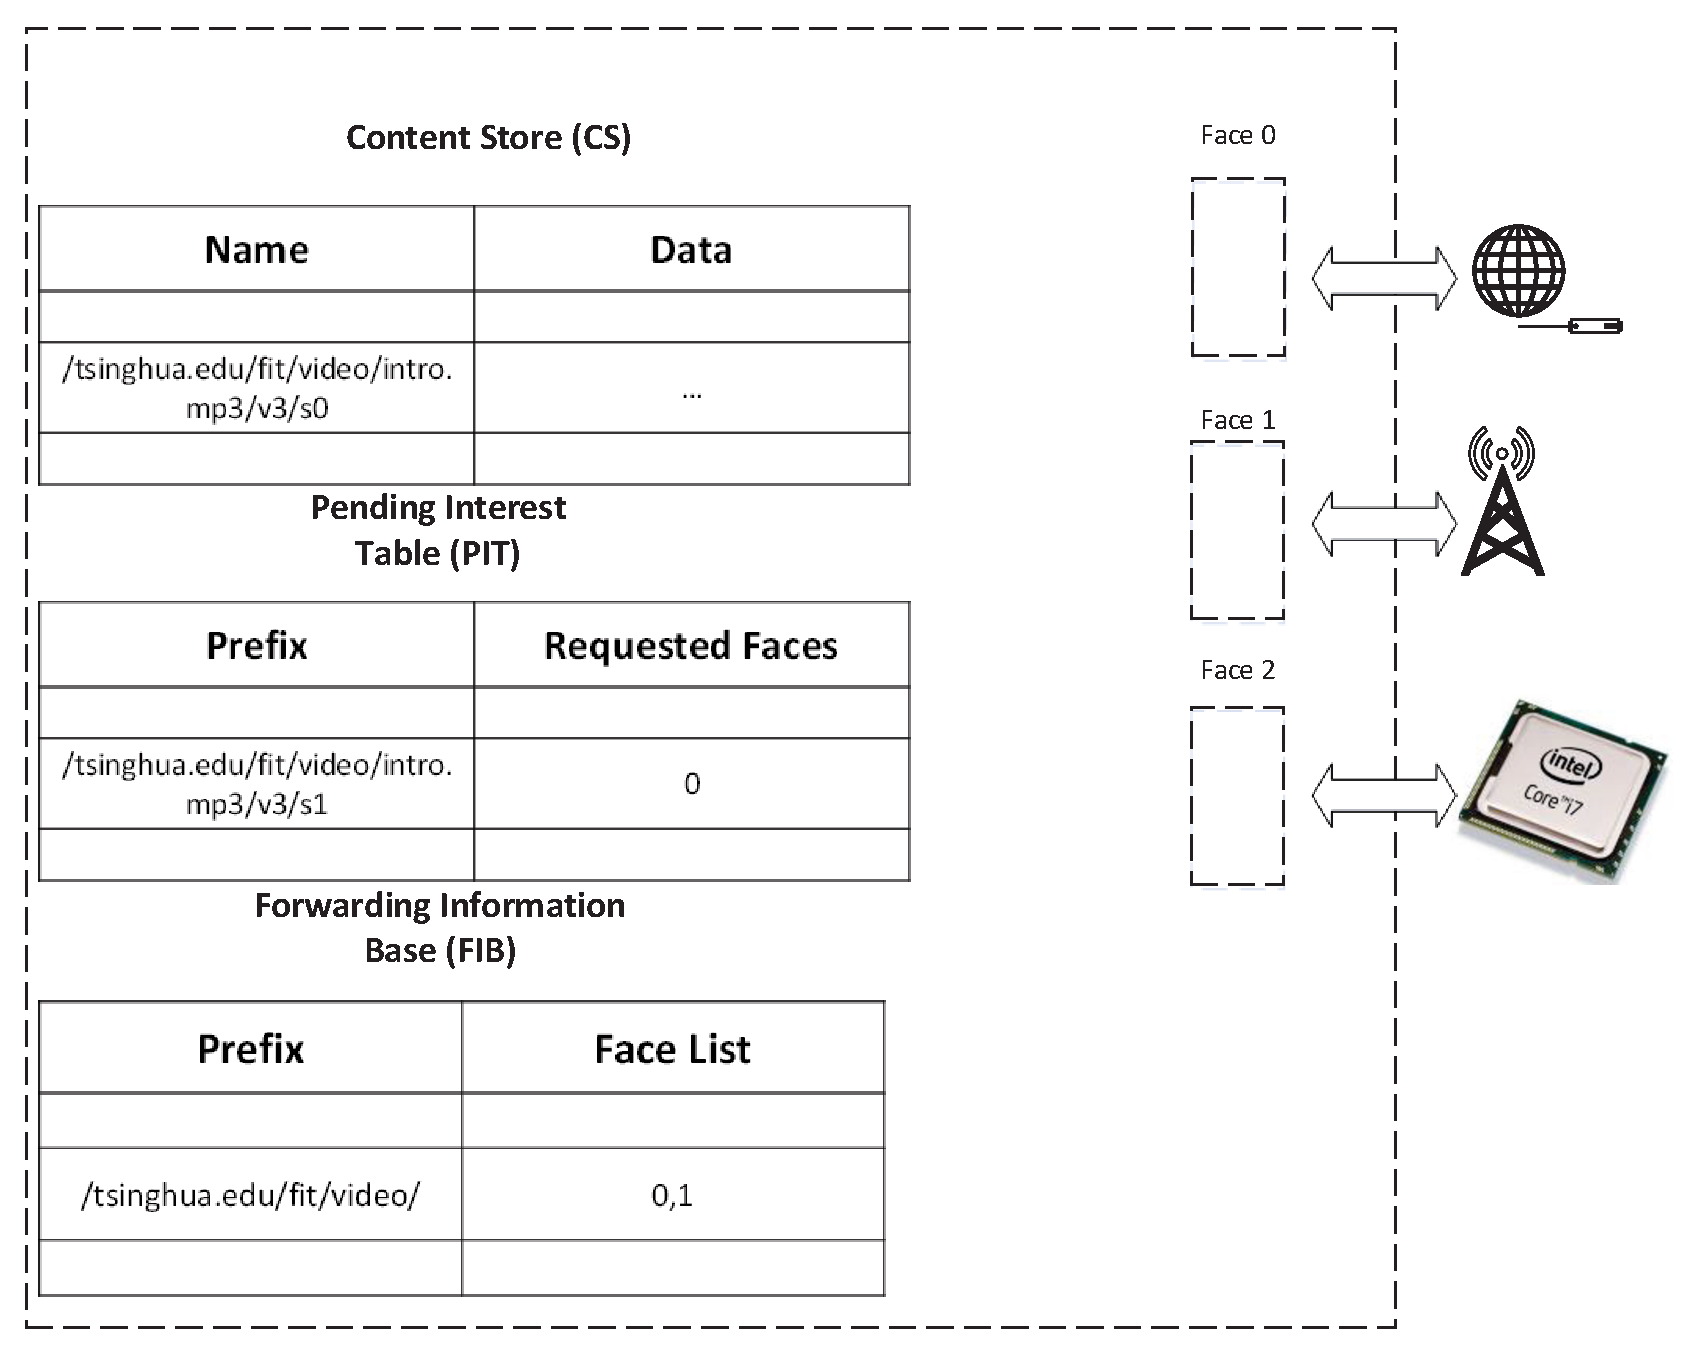
\includegraphics [width=0.8\textwidth]{NDN-stack.eps}
\caption{NDN node}
\label{fig:NDN-node}
\end{center}
\end{figure}

典型的NDN节点处理interest包的流程如下所示:

\begin{enumerate}
\item NDN node接收到被转发的Interest
\item NDN node检查CS看是否有能与interest匹配的数据包,如果找到,则返回该数据包,如果没找到,则继续。
\item 将interest放到PIT表中,并记录它到来的端口
\item 根据最长前缀匹配原则查询FIB表,如果找到,则将interest发送到对应的端口中,如果没找到,则放弃这个interest。
\end{enumerate}

\subsection{命名存储}
\subsubsection{NDN Repository}
在前面章节中,已经介绍了NDN Repo协议,以及基于NSN的存储服务。NDN Repo服务提供了分布式存储服务的以下基本元素:

\begin{itemize}
\item 基本的数据安全性通过NSN进行了双通道保证。通过签名数据保证了数据的安全性,通过签名的命令保证数据操作的安全性
\item Repo服务通过名字来指定具体提供操作对象,因此可以通过相同的前缀来规范同一个服务下的多个repo服务。
\item NSN的规范服务描述文档提供了相对复杂数据操作命令的制定,同时也为客户端操作提供了标准化的接口
\item 基于NDN的CS模块可以作为分布式的数据分发缓存。
\item 以NDN Node的FIB为基础,实际FIB是对网络数据的描述。可以同对本地数据块的描述进行整合。
\item NDN Repo的实现符合了基本的Application Level Framing的概念。\cite{clark1990architectural}。在NDN Repo中挽留过数据直接存储在Repo的后台存储中,Repo以及基于Repo的应用直接操纵网络数据块,节省了应用数据描述与网络数据描述之间的转换。
\end{itemize}

\subsubsection{Data-Centric Storage in Sensornets}
数据中心存储(Data-Centric Storage)\cite{ratnasamy2002ght,shenker2003data}为传感器网络(sensornet)存储设计。它利用哈希结构构建了分布式的数据存储网络。在100,000个节点的拓扑中,数据中心存储可以节约大量的网络负担以及外部内部存储的沟通符合。该结果显示了以命名数据作为网络存储单元给整体存储网络带来的性能优势。

\section{NDSS系统设计}
\subsection{NDSS系统设计原则}
NDSS最主要的设计原则就是节约存储系统在传输数据过程中对同一个数据存储描述与网络描述的多次转换的过程。在典型的分布式存储系统中,例如HDFS基于TCP/IP协议以及posix接口的文件系统,在其传输过程中有两项主要的冗余。一个是上层应用可用的数据描述与可被网络阐述数据描述之间的转换。当网络包到达数据节点,首先需要从网络包中提取出应用层可用的数据来判断是要做出的数据还是操作的命令。另一个冗余是应用层数据描述与本地存储媒介的数据描述。以HDFS为例,当上层应用读取数据时,需要将抽象数据块的具体位置映射到本地实际存储文件系统的具体位置。

在前面的repo-ng中,repo-ng的设计节约了网络数据描述到应用可用数据描述之间的转换过程。而能够节约的本质原因在于通过NDN的数据命名机制对于上层应用来说也是有意义的。

NDSS设计基于前述NSN网络,通过repo-ng的设计,利用命名机制来节约数据描述转换冗余。通过NSN设计,来规范操作安全与规范存储服务可操作性。NDSS设计最重要的一点是通过将NDN的FIB进行改造来统一网络数据与存储数据的描述,同时通过简化网络协议栈来减少由于复杂的网络下层协议带来的传输延迟。

\subsection{命名数据设计}
整合网络与存储的关键在于命名数据设计。NDSS通过命名的数据来统一网络与存储对于数据的描述。当应用操作本地存储的数据时,通过数据的名来对应本地存储媒介的具体位置,而在NDN网络中,则是通过数据的名字来从网络中来获得数据包。NDSS设计是通过数据名字,对于应用来说无差别地获取对应名字的命名数据。但是对于传统的文件系统来说,posix对应用提供统一的api,在下层针对不同系统,对于api来进行不同的操作与转化,而NDN网站是直接通过CS或者FIB来进行数据查找。

在NDSS设计中,数据的获取与返回在抽象层面上统一。Interest中包含需要获取命名数据的名字前缀以及规定数据选择条件的selector。在NDSS系统中提出了新的一种selector,\textit{priority}。网络和本地存储被看做两个不同的数据源,而priority选择子用来控制优先选择哪个数据源的数据。

在NDN与NSN中,数据包必须要进行签名,但是如果应用获取的是本地生成并且在本地存储的数据,则没有必要去验证这个数据。在NDSS的数据包中,通过\textit{local}标签来表述这个数据一直呆在本地。如果是外来的数据转发到本地,或者本地的数据被转发到另外一个主机,\textit{local}标签会被置为false。

\subsection{NDSS节点模型}
NDSS数据传输依靠数据消费者驱动。NDSS借用了NSN的数据传输机制以及远程服务调用机制。数据请求与数据响应,无论是本地数据还是网络数据,都依靠的是interest和data模式。在NDSS中,interest不仅可以转发到网络中,还可以传递给下层本地存储结构。FIB被修改为Local and Forwarding Information Base(LFIB)。NDSS的节点结构如图\ref{fig:NDSS-node}所示。

在图\ref{fig:NDSS-node}中可以看到,NDSS依然采用了NDN的CS与PIT结构,CS作为数据的缓存,PIT记录未被响应的interest的来源端口与去向端口。在NDSS节点中,整合网络数据与本地数据的关键为LFIB结构。与NDN的FIB相比,LFIB增加了本地索引列。对于LFIB的一条项目,不仅需要记录需要向哪个端口获取,还有记录它在本地的位置,即该数据块在本地存储介质上的位置索引。对于主流块数据存储介质,LFIB可以直接记录在块存储介质的位置。当NDSS数据请求来时,可以通过LFIB同时查询该数据在网络与本地存储的位置。

\begin{figure}[!htb]
\begin{center}
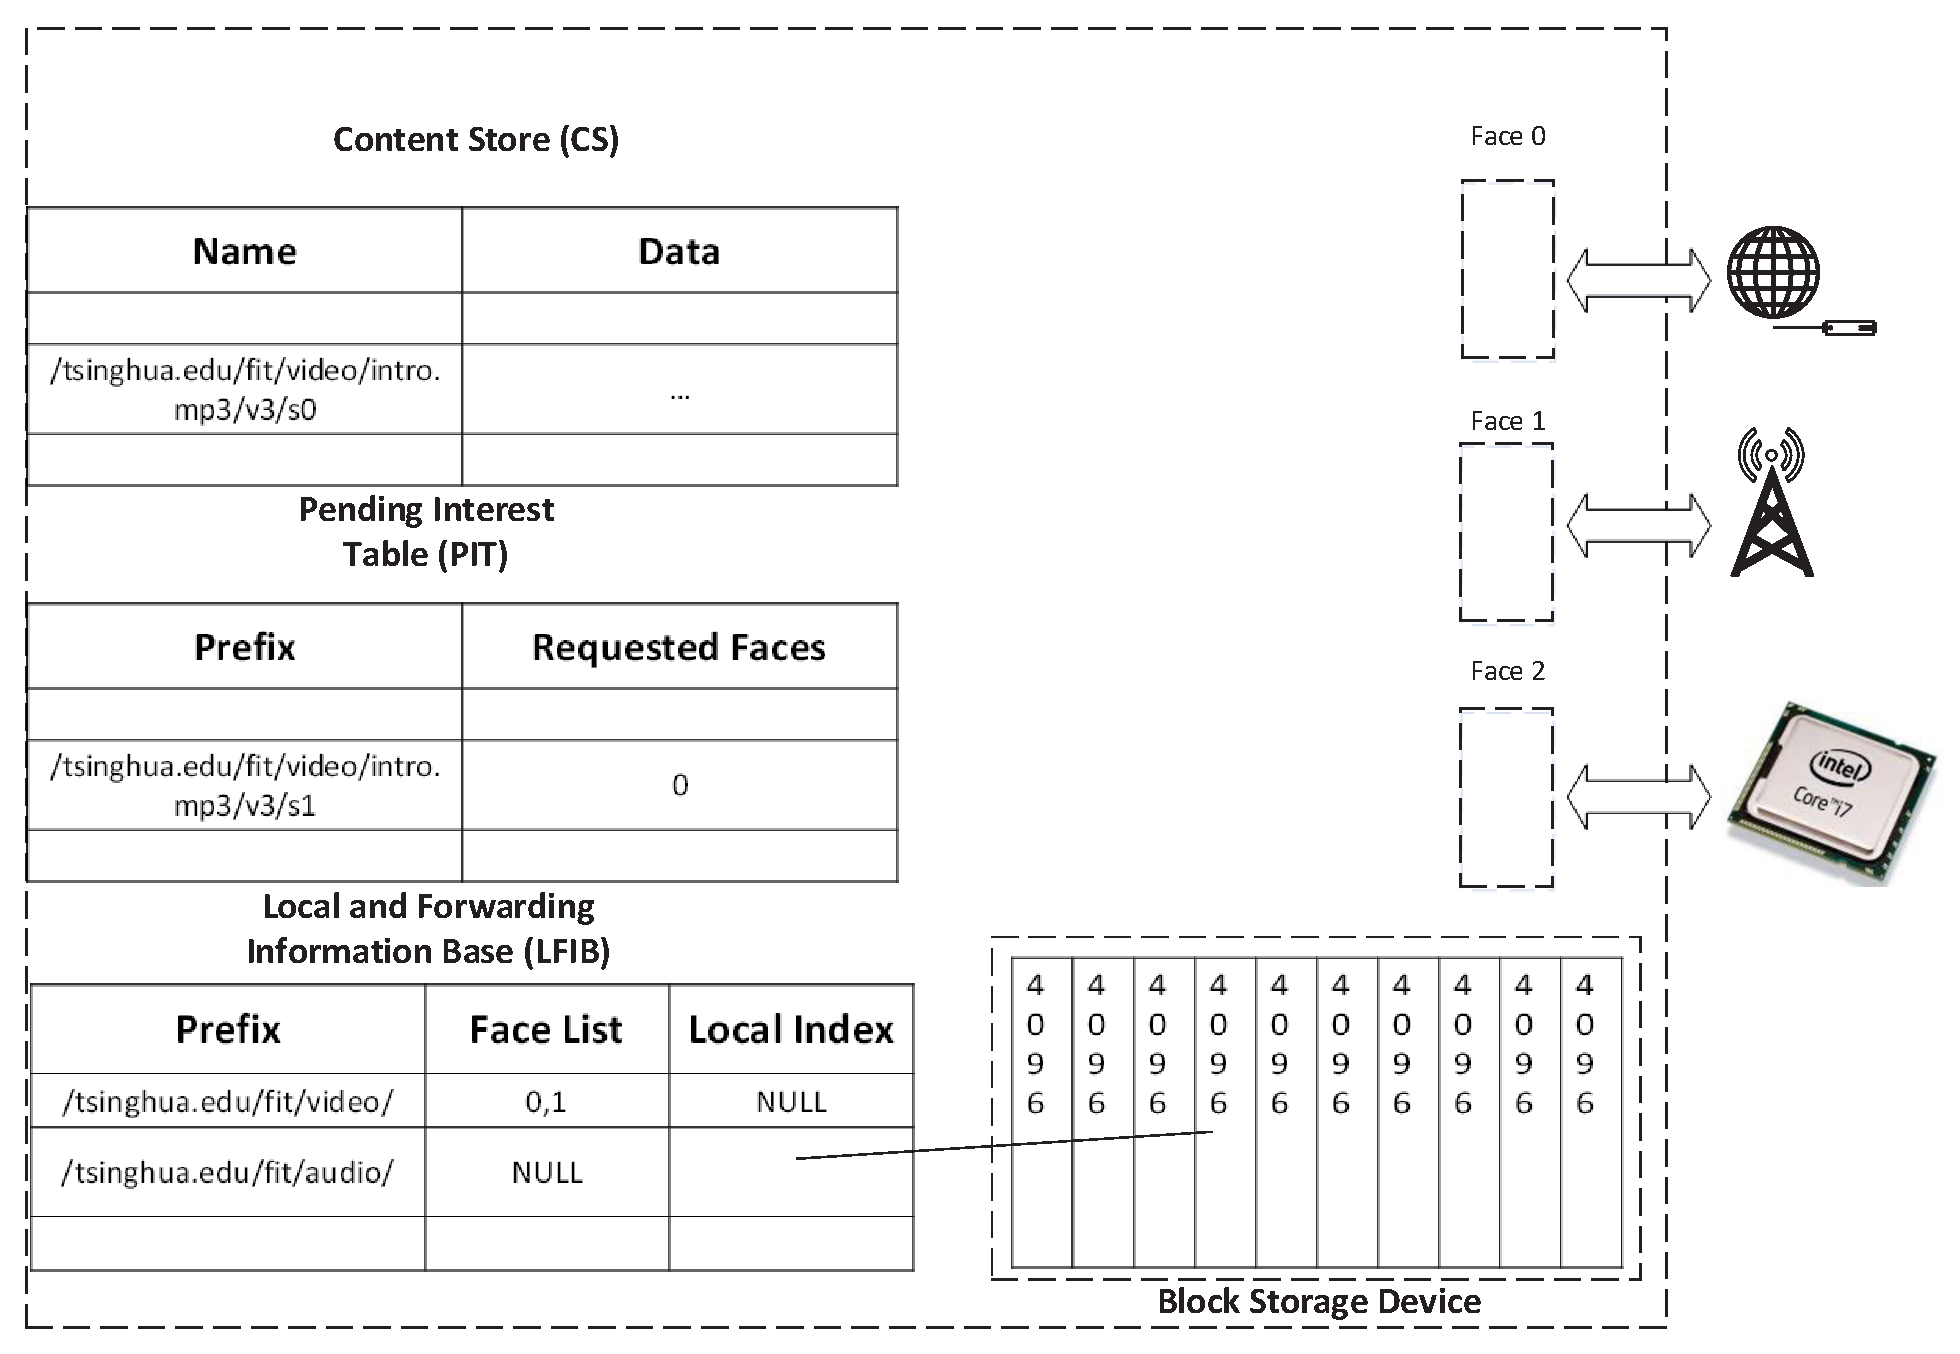
\includegraphics [width=0.8\textwidth]{NDSS-stack.eps}
\caption{NDSS node}
\label{fig:NDSS-node}
\end{center}
\end{figure}

\subsection{NDSS操作模型}
NDSS基于NSN的的存储服务搭建,对于远程单点数据操作,NDSS服务基于NSN的NDN Repo协议。NDSS操作可以分为两类:数据获取类与数据更新类。对于数据获取类操作,根据NDSS节点模型,发送对应数据前缀的interest即可根据LFIB获取数据。对于数据更新类操作,包括数据的插入与删除。需要NDSS节点支持NSN的Repo服务协议,需要将NSN Repo服务命令转换成操作数据存储介质的操作。

NDSS从本质上来说是一个元数据分布式的存储系统,元数据信息即LFIB分布在各个NDSS节点之中。NDSS为一组松散的数据服务,通过名字前缀来划分数据操作作用域,当NDSS节点需要普遍的支持数据获取操作,选择性的可以支持数据更新操作。

\subsection{NDSS扁平网络协议栈}
NDN目前的实现是覆盖网络,通常是基于TCP或者UDP。NDNLP\cite{shi2012ndnlp}提出了一种介于NDN与以太网之间的传输协议,该协议主要关注与将NDN网络包进行分帧,并在以太网上进行传输,在一定程度上保持了消息的有序性。但是NDN下面复杂的协议栈增加了数据传输的网络冗余。以CCNx为例,命名数据需要被下层网络分片并重新组合。此外在网络包传输过程中,会经过NDN层面与IP层面两次路由。网络流量控制,拥塞控制以及可靠传播可以在NDN网络内部得到解决,NDN本身运行并不需要下层的传输层以及网络层。在\cite{clark1990architectural}中,应用层帧利用统一的网络协议栈以达到高效的数据操作。NDSS将NDN直接建立在以太网协议栈上以实现Appliaction Data Unit(ADU)来减小网络处理冗余。与NDN覆盖网比较,NDSS采用了underlay的设计。NDSS的网络协议栈结构如图\ref{fig:NDSS-underlay}所示。

\begin{figure}[!htb]
\begin{center}
\includegraphics [width=0.8\textwidth]{underlay.eps}
\caption{NDSS underlay网络协议栈}
\label{fig:NDSS-underlay}
\end{center}
\end{figure}

与TCP/IP网络相比,underlay网络设计只需保证跳之间的网络传输,因此在NDSS underlay网络中,MAC地址同样也不需要,只需要知道NDN前缀就可以,在NDSS实现中,MAC头中的地址部分可以去掉。

\subsection{NDSS传输流程}
NDSS设计的初衷是节约在数据传输中的冗余。NDSS节点模型节约了网络数据与存储数据之间的转换冗余。NDSS网络模型节约了节点与节点之间,网络包转发的冗余。NDSS几种数据传输流程如下所示:

\subsubsection{本地应用获取本地数据}
\begin{enumerate}[step 1.]
\item 应用发送特定的数据请求
\item 检查CS是否有匹配请求的数据。如果找到,返回数据并结束流程。
\item 检查PIT是否有相同的数据请求,如果找到,则在PIT表增加对应项,并结束流程
\item 检查LFIB表,如果命中,根据priority选择子来选择是本地数据还是网络数据。假设后面流程是基于本地数据。
\item 通过LFIB中记录的数据索引直接选中数据块
\item 删除PIT中对应项目
\item 把返回数据块加入CS
\item 应用得到数据
\item 检查数据包中的local标签,如果local标签是false,则应用应该验证该数据。
\end{enumerate}
\subsubsection{本地应用获取外部数据}
\begin{enumerate}[step 1.]
\item 应用发送特定的数据请求
\item 检查CS是否有匹配请求的数据。如果找到,返回数据并结束流程。
\item 检查PIT是否有相同的数据请求,如果找到,则在PIT表增加对应项,并结束流程
\item 检查LFIB表,如果命中,根据priority选择子来选择是本地数据还是网络数据。假设后面流程是基于网络数据,将interest发送到对应端口。
\item 等待数据返回
\item 从以太网帧中直接提取对应数据包
\item 删除PIT中对应项目
\item 把返回数据块加入CS
\item 应用得到数据,并验证数据签名
\item 如果上层应用要将数据写入本地存储,则可以将该数据直接写入存储介质的数据块之上。数据的位置索引添加到对应的LFIB之中。
\end{enumerate}

\subsubsection{NDSS节点处理外部interest}
\begin{enumerate}[step 1.]
\item NDSS接收到外部转发的interest。
\item 检查CS是否有匹配请求的数据。如果找到,返回数据并结束流程。
\item 检查PIT是否有相同的数据请求,如果找到,则在PIT表增加对应项,并结束流程
\item 检查LFIB表,如果命中,根据priority选择子来选择是本地数据还是网络数据。假设后面流程是基于本地数据。
\item 通过LFIB中记录的数据索引直接选中数据块
\item 将本地数据块的local标签设置为false
\item 根据PIT记录返回查找到的数据,删除PIT中对应项目
\item 把返回数据块加入CS
\end{enumerate}

\section{NDSS系统实现}
NDSS实现主要包括两部分,一个是NDSS节点模型和NDSS下层网络协议栈。在本节中,实现并测试了NDSS的下层网络协议栈,提出了NDSS节点模型的实现设计。

\subsection{NDSS节点模型实现设计}
在传统的系统中,上层应用通过文件系统或网络套接字来获取数据。在Linux系统中,数据可以通过\textit{read()}或\textit{write()}方法通多读写文件描述符(file descriptor)来获取。在NDSS中,数据获取的单位直接是命名数据块。如果上层应用想以文件为单位操作数据,可以在NDSS块级别数据操作上基础上建立类似于NDNFS\cite{shangndnfs}的文件系统。

基于Linux的NDSS实现设计如图\ref{fig:NDSS-imp}所示。块存储设备挂载在VFS之上。通过glibc利用\textit{read()}和\textit{write()}方法直接读取块设备和原始套接字。原始套接字是用来跳过TCP/IP协议栈直接读取以太网帧。

\begin{figure}[H]
\begin{center}
\includegraphics [width=0.4\textwidth]{NDSS-imp.eps}
\caption{NDSS节点实现设计}
\label{fig:NDSS-imp}
\end{center}
\end{figure}

\subsection{网络协议栈实现与实验评估}
NDSS利用以太网作为下层传输协议。为了适应NSN及上层的NDN协议,有两个问题需要解决:命名数据块的大小以及去掉以太网头。

以太网不提供网络包的分段功能,通常MTU的大小为1500。但是一般命名数据块大小都要大于默认的MTU大小。在现在的以太网卡一般都支持Jumbo Frame(巨大帧)。通常Jumbo Frame可以承载7000以上的MTU。

在一般模式下,以太网会抛弃没有Mac头的以太网帧,因为以太网会根据Mac头中的目的地址去过滤以太网包。但是现代操作系统一般支持promiscuous模式,在该模式下,任何以太网包都不会被过滤掉。

实验评估中测试了两个主机直连模式下underlay网络的数据吞吐速度。数据吞吐速度利用CCNx的ccngetfile工具进行测试。结果如图\ref{fig:1hop}所示。

\begin{figure}[H]
\begin{center}
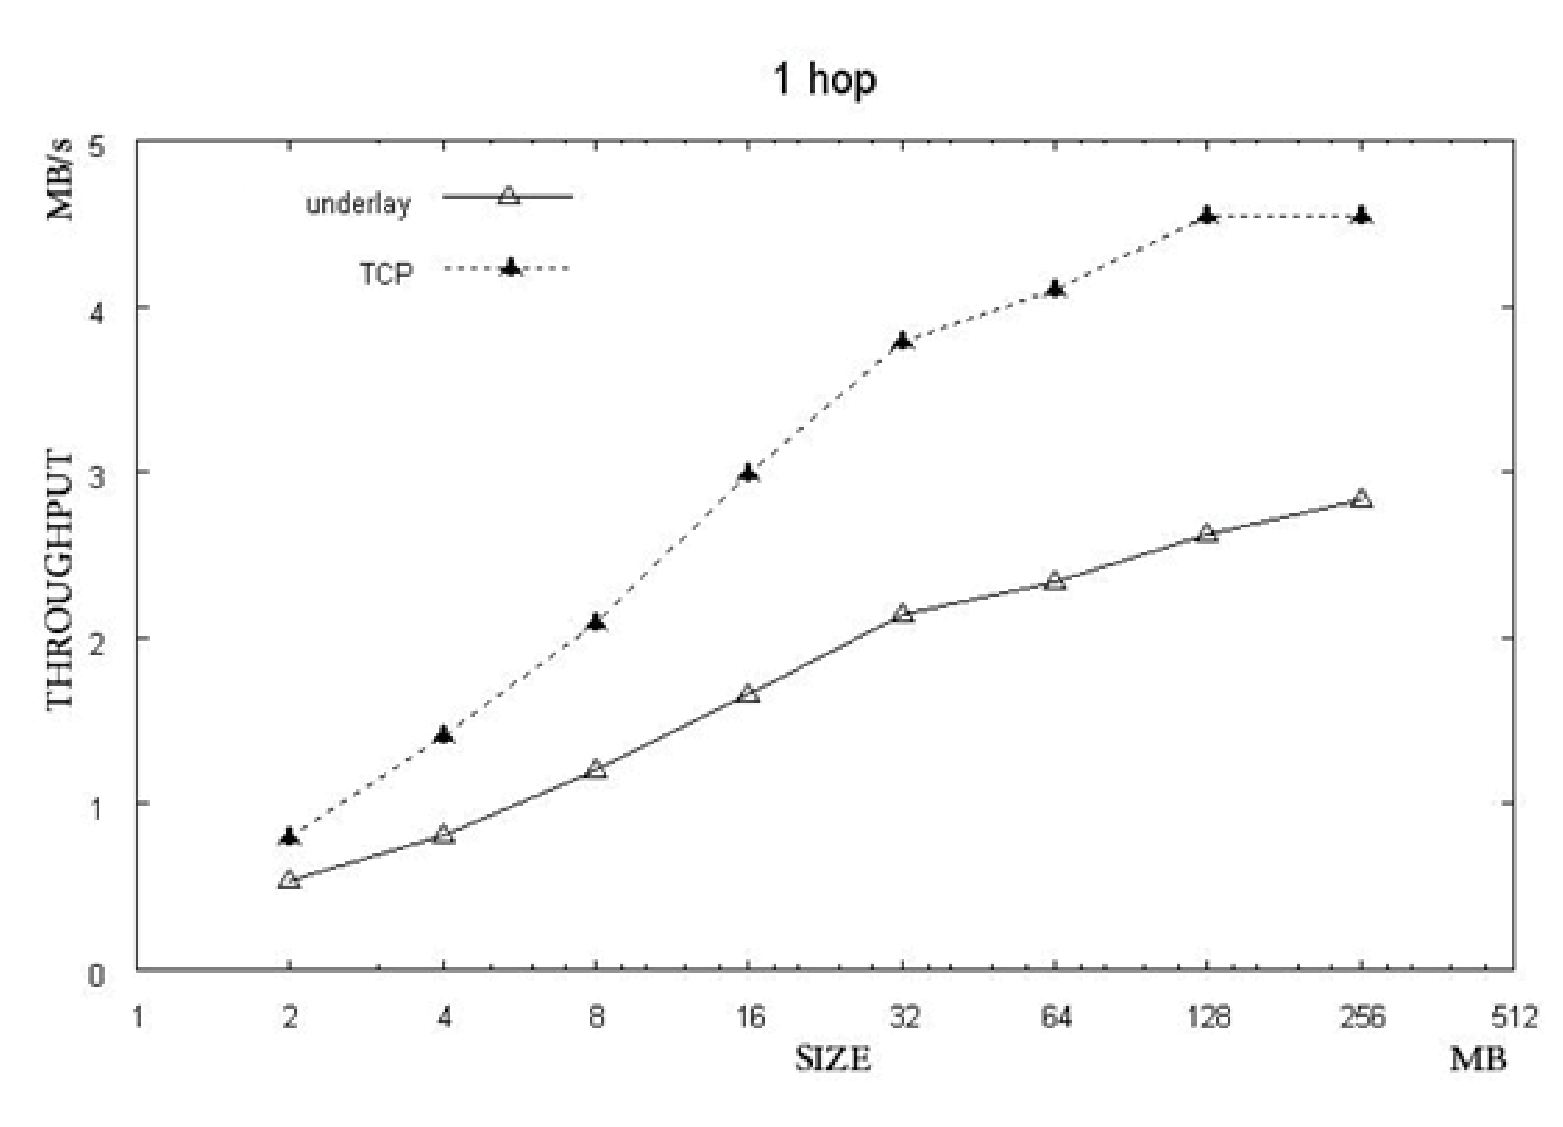
\includegraphics [width=0.5\textwidth]{1hop.eps}
\caption{underlay单跳吞吐速度}
\label{fig:1hop}
\end{center}
\end{figure}

由于linux系统中,TCP/IP协议栈在内核中进行了大量的优化。而\textit{raw socket}以及\textit{promiscuous}的优化程度相对一般,所以可以看到比较合理的性能下降。

\section{总结}
NDSS的设计理念源自于应用层帧的原则(application level framing),通过在应用层定义数据存储与网络的表现形式减小在数据传输与存储当中的冗余。NDSS的核心设计为同过LFIB统一网络与本地存储数据描述,通过扁平网络协议栈来减少网路传输冗余,通过NSN来提高存储节点的可操作性。在未来工作中,会继续实现NDSS的节点模型以及优化扁平协议栈以提高NDSS系统的数据效率。
